\chapter{Figuras complementarias}
\label{anx:figuras}

Este anexo reúne las figuras que respaldan afirmaciones del cuerpo sin recargarlo. Cada una se cita en su sitio; aquí se agrupan por lo que sostienen: primero el mecanismo sobre SPY, después el panel.

\section{Mecanismo sobre SPY}
\label{anx:fig-spy}

\begin{figure}[htbp]
\centering
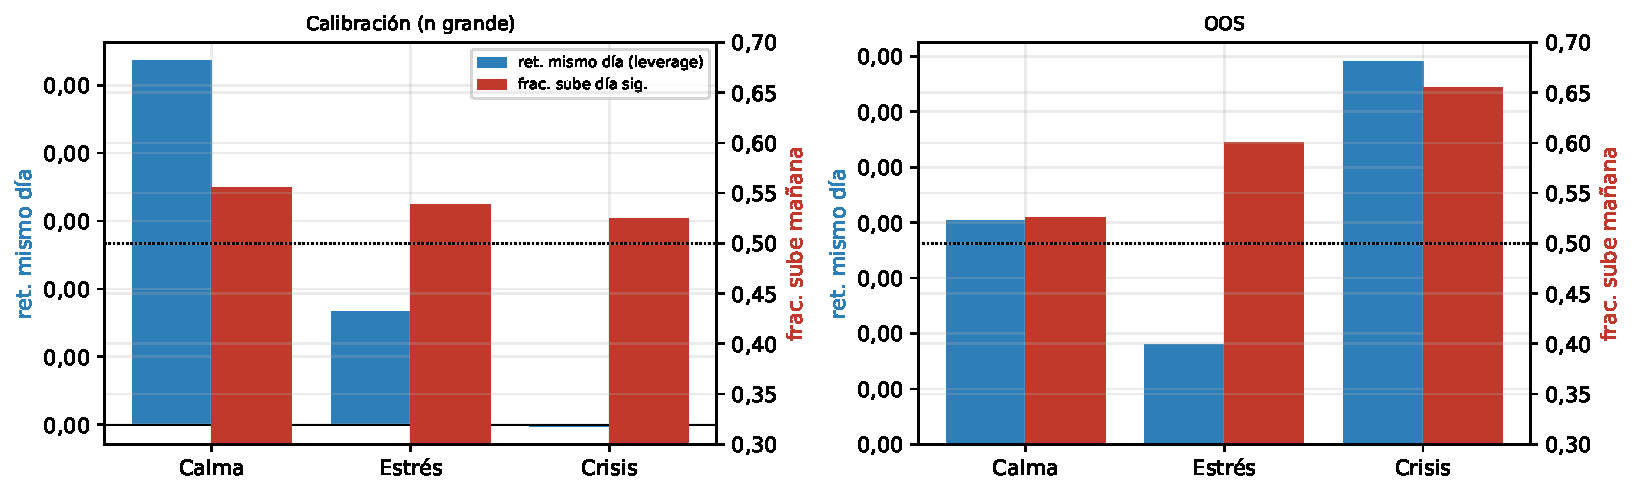
\includegraphics[width=0.80\textwidth]{figuras/cap4_anexo_regimen_direccion}
\caption{Matriz régimen $\times$ dirección sobre SPY, en calibración y fuera de muestra. El régimen coincide con la caída del mismo día, pero no anticipa el signo del siguiente: el \emph{leverage} que explota RAM es contemporáneo, no predictivo.}
\label{fig:anx-regimen-dir}
\end{figure}

\begin{figure}[htbp]
\centering
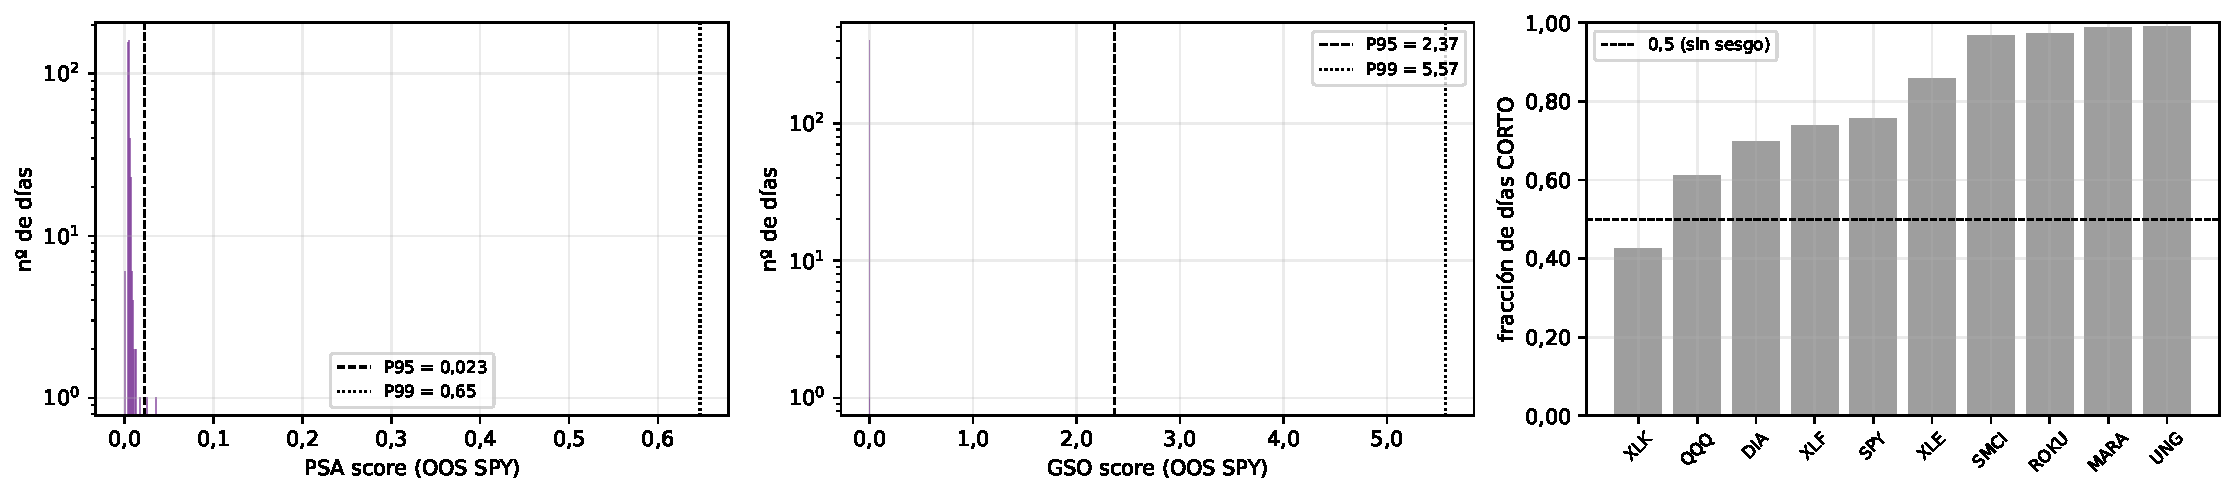
\includegraphics[width=0.80\textwidth]{figuras/cap4_anexo_psa_gso}
\caption{Scores de PSA y GSO frente a su umbral ex ante, junto al sesgo casi constante del agente. Los dos detectores rara vez cruzan el umbral porque el agente apenas cambia de posición: están dormidos sobre este activo, no rotos.}
\label{fig:anx-psa-gso}
\end{figure}

\begin{figure}[htbp]
\centering
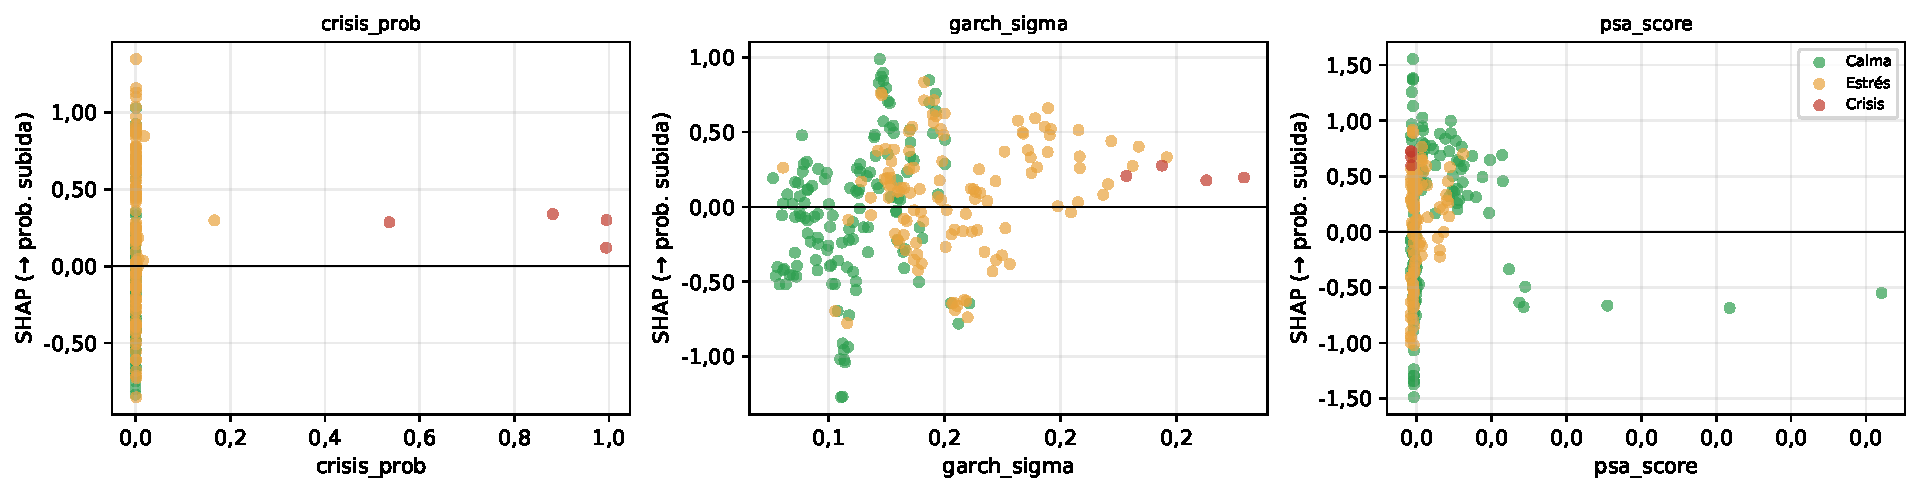
\includegraphics[width=0.85\textwidth]{figuras/cap4_anexo_shap_dependency}
\caption{Dependencia SHAP de las señales de STRATA en el aprendiz: cómo cambia su contribución al variar cada \emph{score}. El modelo no las usa de forma plana, las modula según el régimen.}
\label{fig:anx-shap-dep}
\end{figure}

\begin{figure}[htbp]
\centering
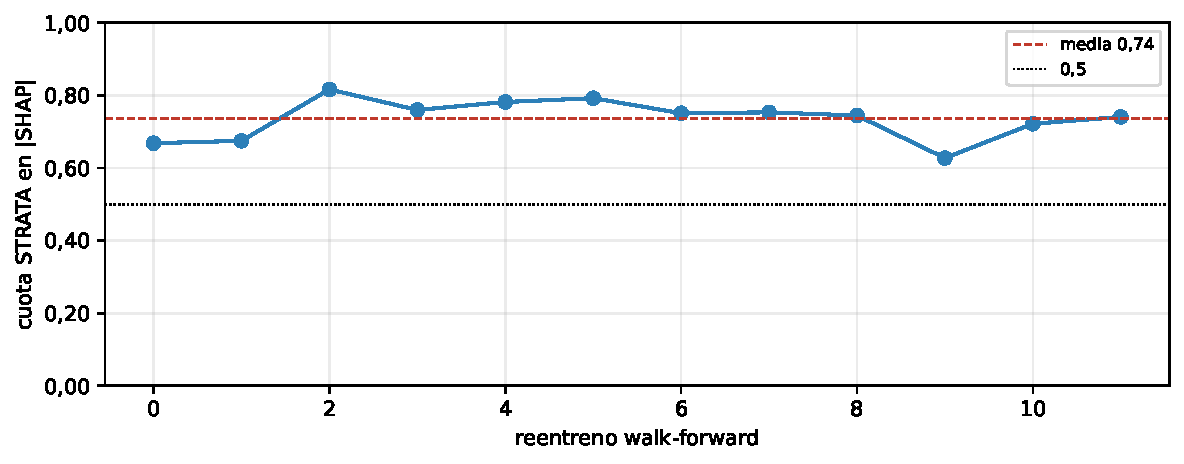
\includegraphics[width=0.74\textwidth]{figuras/cap4_anexo_shap_rodante}
\caption{Cuota de importancia de las señales de STRATA a lo largo del tiempo, por reentreno. Se mantiene mayoritaria en toda la ventana: el aprendiz se apoya en STRATA de forma estable, no en un tramo afortunado.}
\label{fig:anx-shap-rodante}
\end{figure}

\begin{figure}[htbp]
\centering
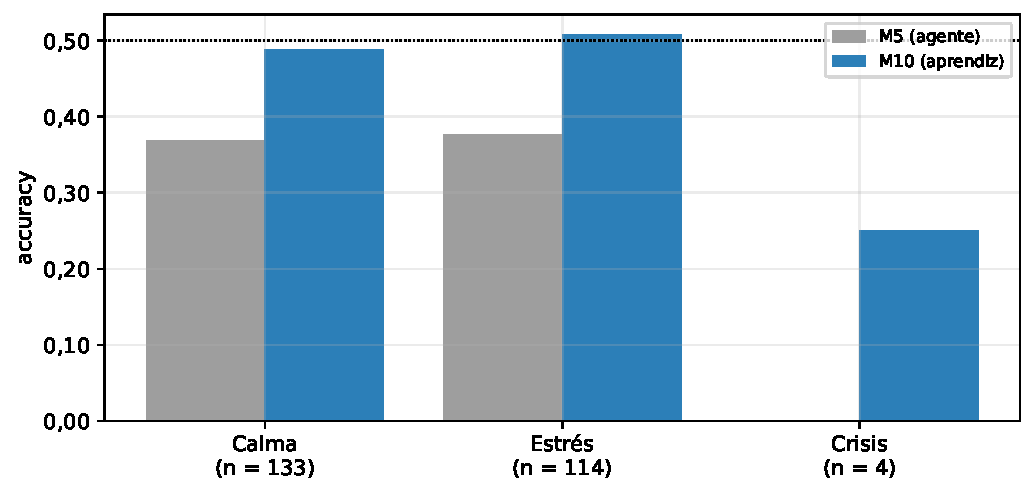
\includegraphics[width=0.72\textwidth]{figuras/cap4_anexo_confusion_m10_regimen}
\caption{Acierto del agente (M5) y del aprendiz (M10) por régimen, sobre SPY. El aprendiz corrige sobre todo donde el agente más se equivoca.}
\label{fig:anx-confusion-m10}
\end{figure}

\section{Panel de diez activos}
\label{anx:fig-panel}

\begin{figure}[htbp]
\centering
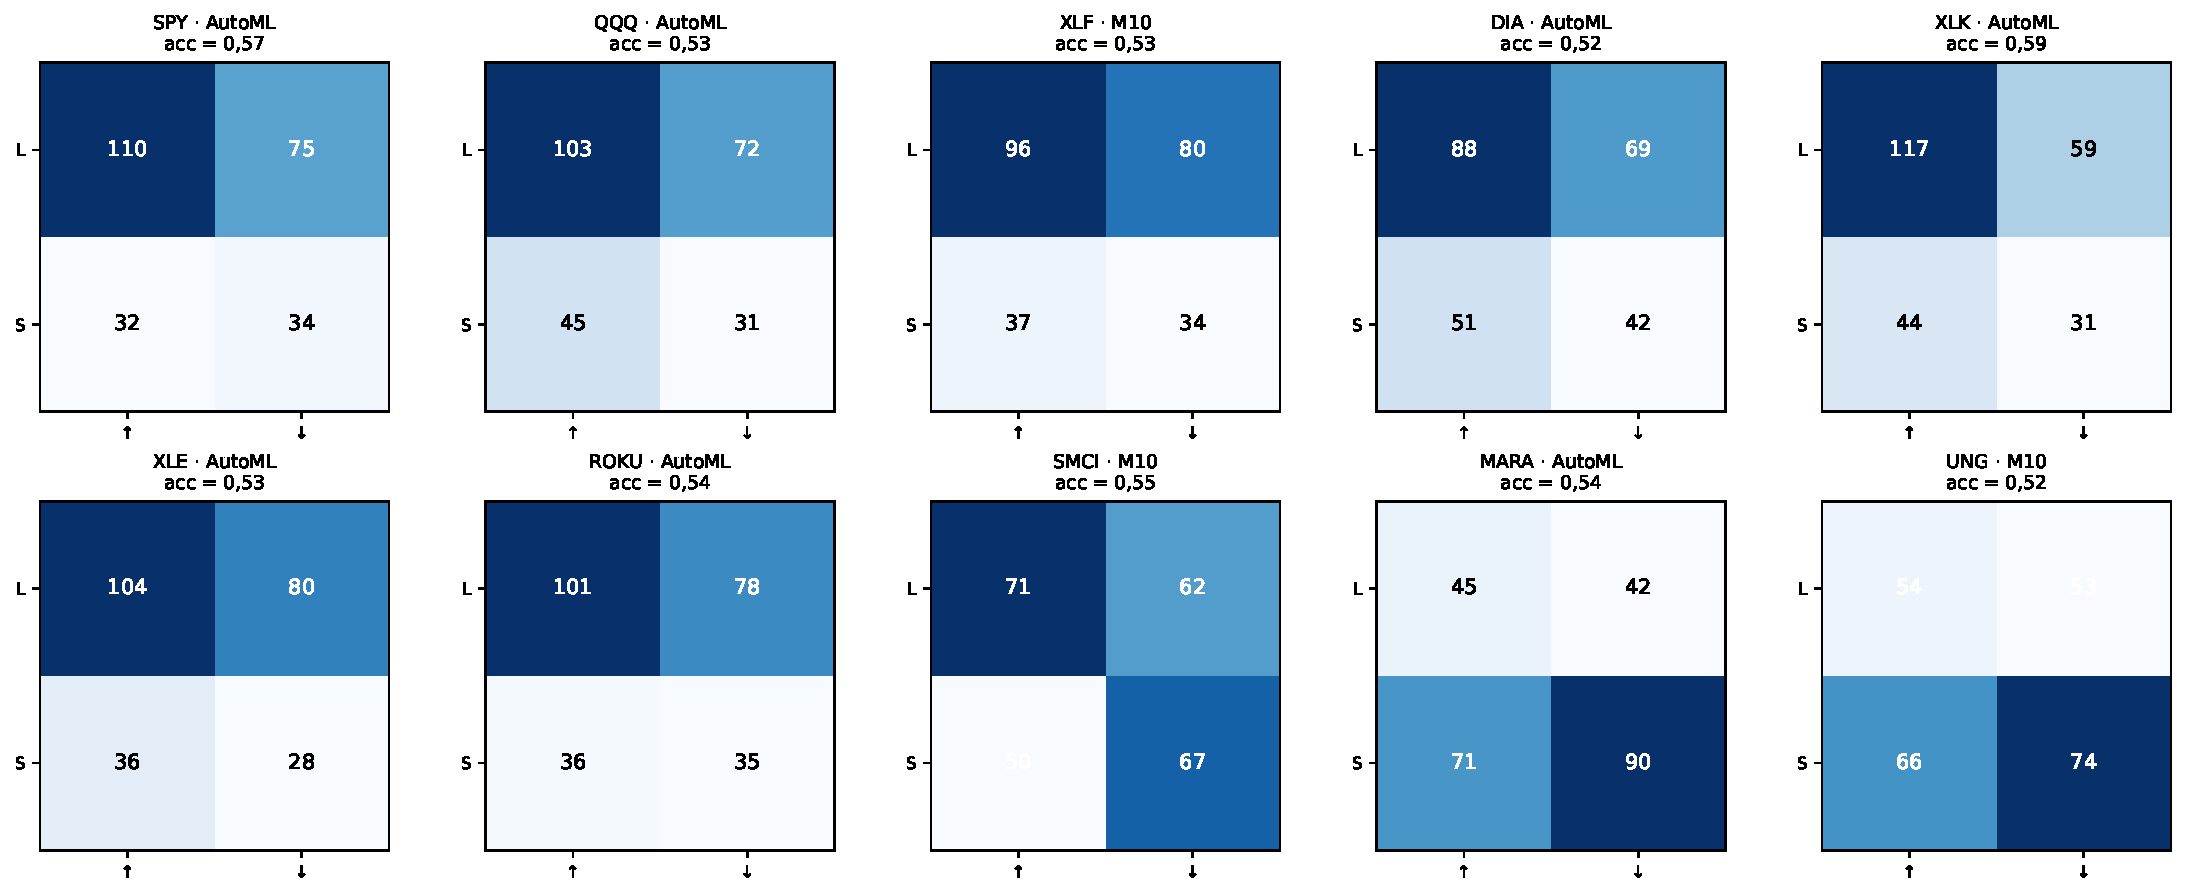
\includegraphics[width=0.92\textwidth]{figuras/cap4_anexo_confusion_panel}
\caption{Matrices de confusión de la mejor derivada de STRATA en cada activo. Enseñan el reparto de aciertos y fallos detrás de cada accuracy del panel.}
\label{fig:anx-confusion-panel}
\end{figure}

\begin{figure}[htbp]
\centering
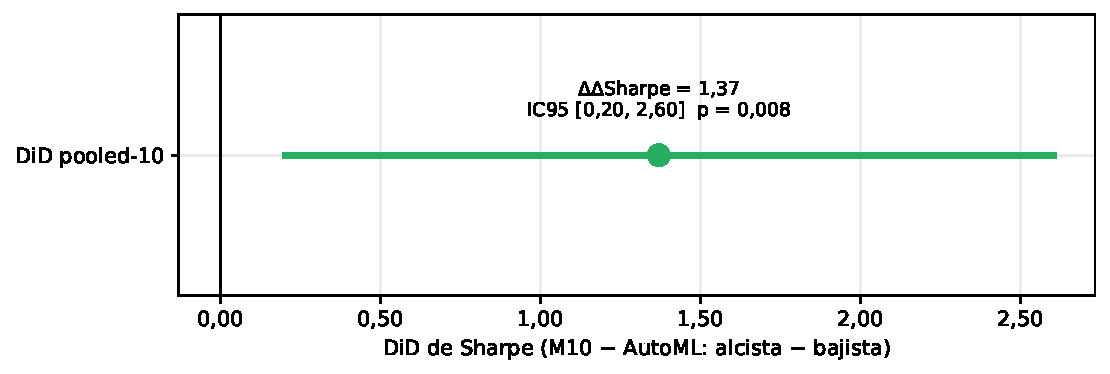
\includegraphics[width=0.78\textwidth]{figuras/cap4_anexo_did}
\caption{Contraste de diferencia en diferencias de la complementariedad por régimen: $\Delta\Delta$Sharpe \emph{pooled-10} de M10 frente a AutoML entre mercado alcista y bajista, con su intervalo al $95\%$. El intervalo excluye el cero ($+1{,}37$, $p = 0{,}008$): la complementariedad es significativa sobre el panel, no en SPY solo.}
\label{fig:anx-did}
\end{figure}

\begin{figure}[htbp]
\centering
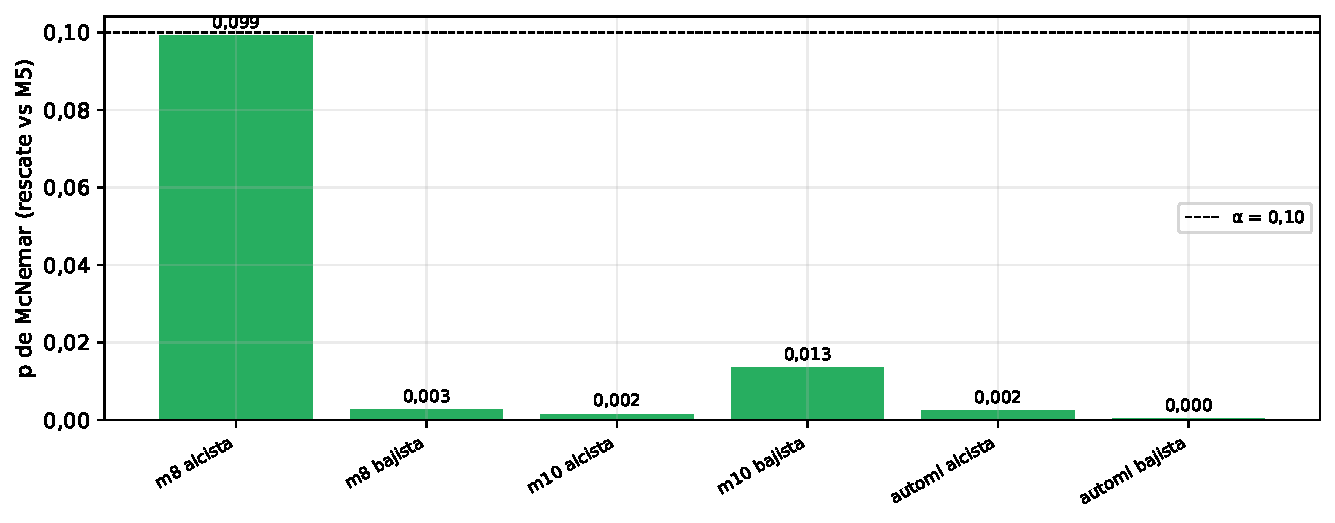
\includegraphics[width=0.78\textwidth]{figuras/cap4_anexo_mcnemar}
\caption{$p$ de McNemar del rescate frente al agente, por estrategia y régimen, con el nivel $\alpha = 0{,}10$ marcado. El rescate en acierto es significativo en los dos regímenes.}
\label{fig:anx-mcnemar}
\end{figure}

\begin{figure}[htbp]
\centering
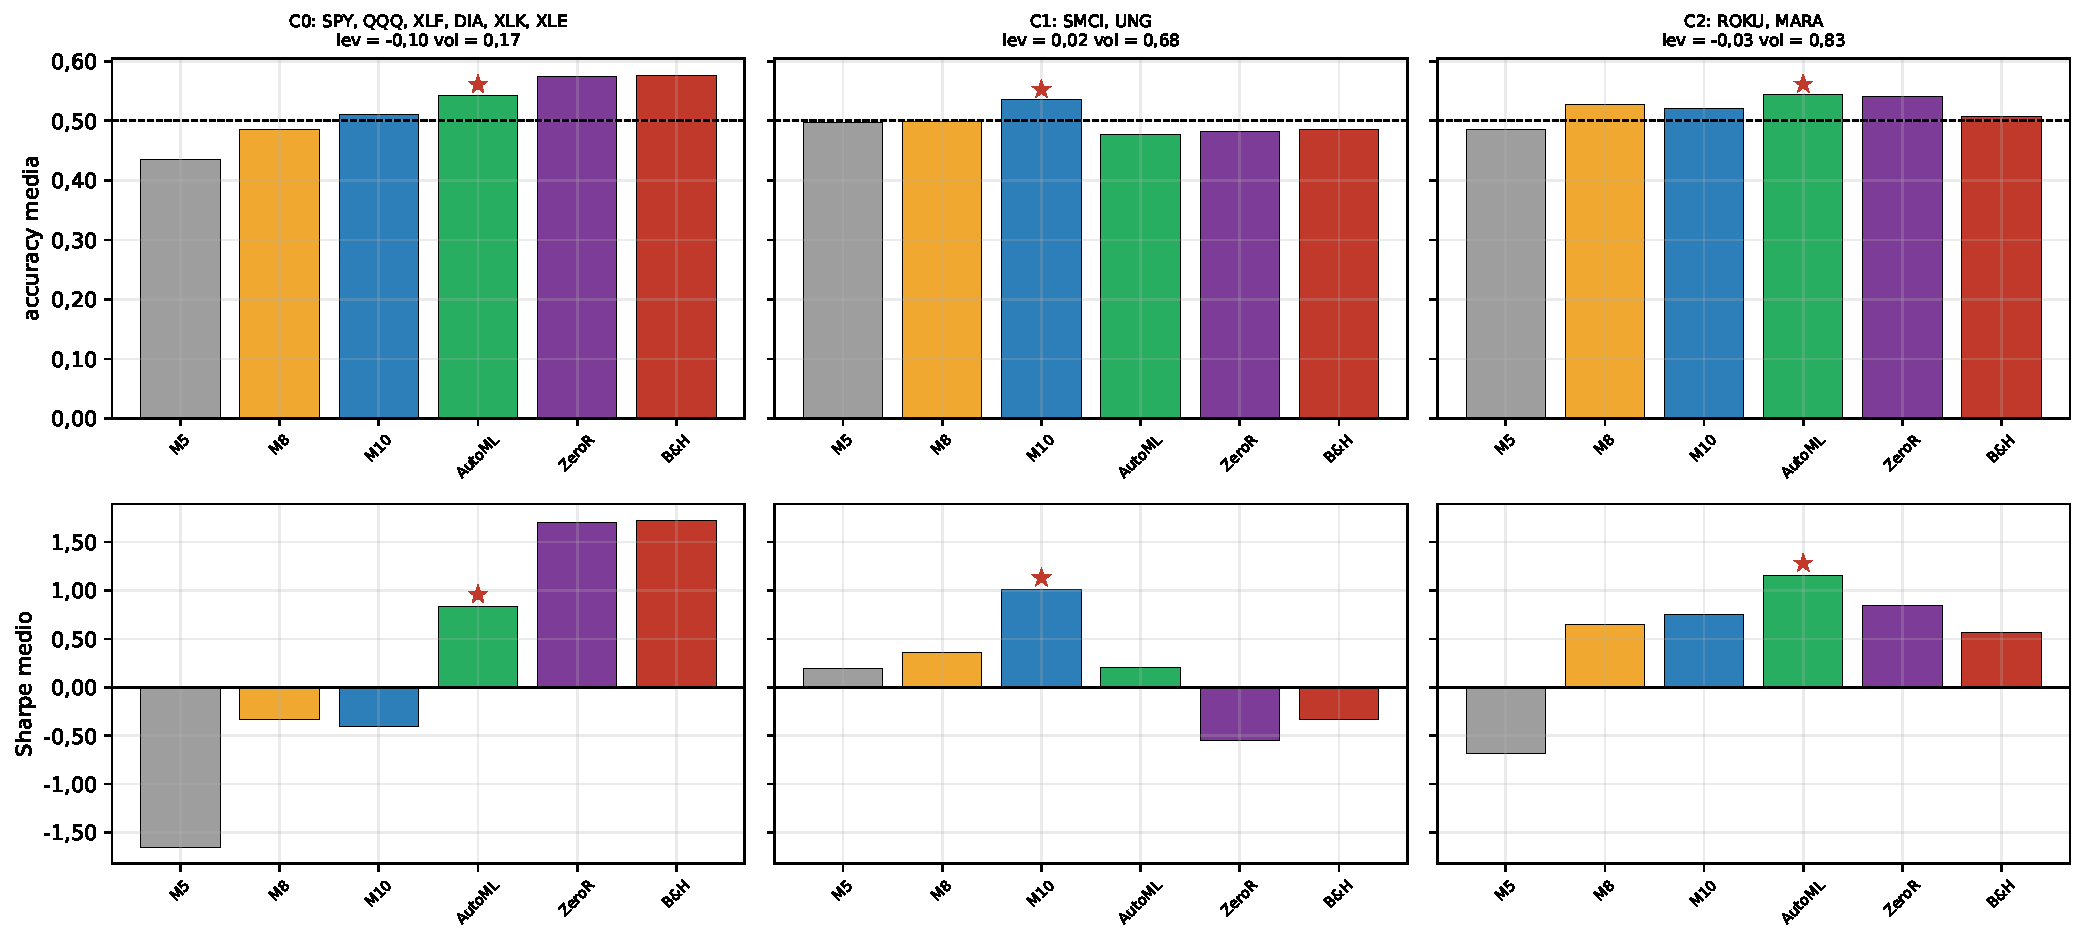
\includegraphics[width=0.85\textwidth]{figuras/cap4_anexo_grupos}
\caption{Accuracy y Sharpe medios por estrategia dentro de cada grupo del clustering. Cada grupo se rescata por un canal distinto, coherente con su naturaleza.}
\label{fig:anx-grupos}
\end{figure}

\begin{figure}[htbp]
\centering
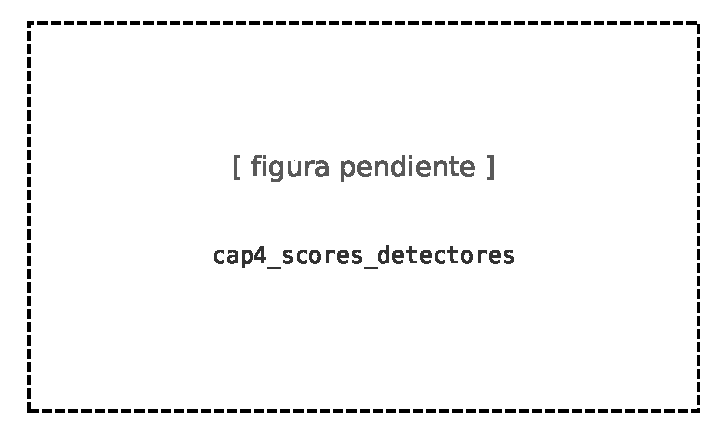
\includegraphics[width=0.74\textwidth]{figuras/cap4_scores_detectores}
\caption{Distribución de los \emph{scores} de RAM, PSA y GSO sobre el OOS de SPY, con su umbral de disparo marcado (RAM $\tau = 0{,}50$, PSA $P_{95} = 0{,}023$, GSO $P_{95} = 2{,}371$). El \emph{score} de RAM es bimodal y cruza el umbral con frecuencia; los de PSA y GSO se acumulan muy por debajo del suyo, de ahí que apenas disparen.}
\label{fig:mp-scores-detectores}
\end{figure}

\begin{figure}[htbp]
\centering
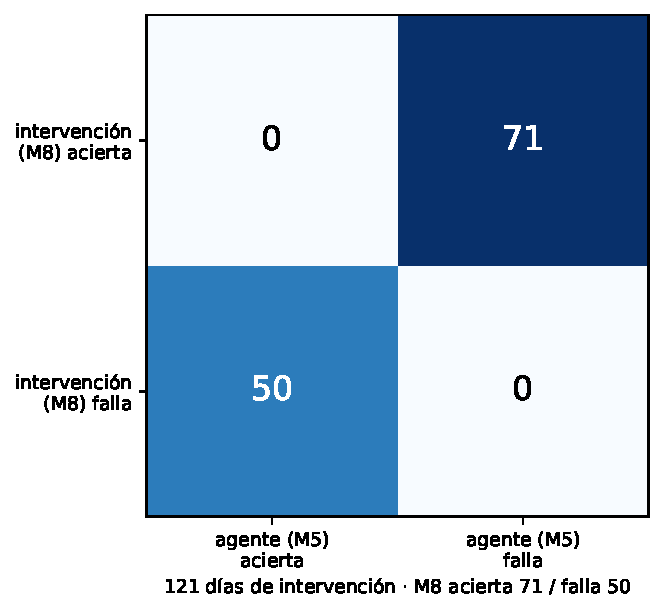
\includegraphics[width=0.7\textwidth]{figuras/cap4_confusion_spy}
\caption{Matriz de confusión de la intervención sobre SPY: dirección del agente (M5) frente a dirección tras intervenir (M8), sobre las $121$ intervenciones. La diagonal de rescate ($71$ aciertos de la intervención cuando el agente fallaba) supera a la de daño ($50$).}
\label{fig:mp-confusion-spy}
\end{figure}

\begin{figure}[htbp]
\centering
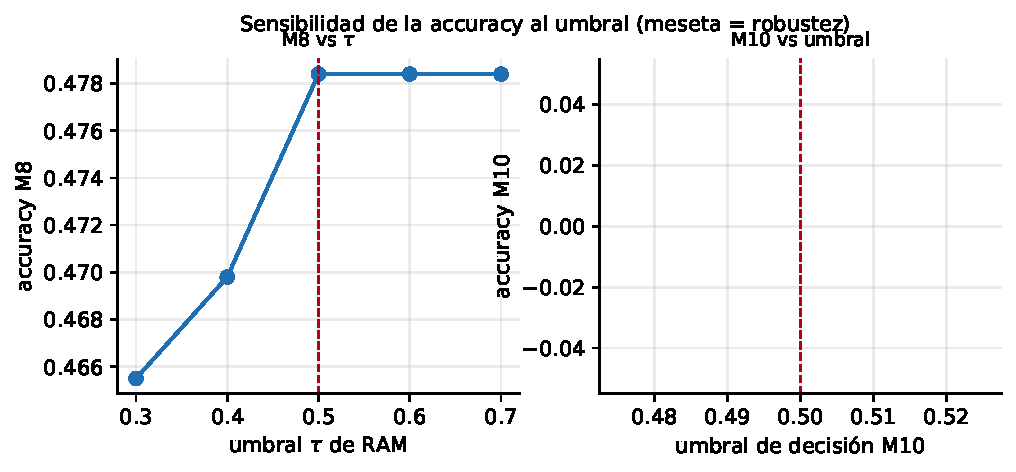
\includegraphics[width=0.74\textwidth]{figuras/cap4_sensibilidad_umbrales}
\caption{Sensibilidad de la accuracy al umbral de decisión sobre SPY: M8 frente a $\tau$ del detector RAM y M10 frente a su umbral de probabilidad. Las dos curvas son planas en una meseta alrededor del valor canónico (marcado), señal de robustez y no de ajuste a un punto.}
\label{fig:mp-sensibilidad}
\end{figure}

\begin{figure}[htbp]
\centering
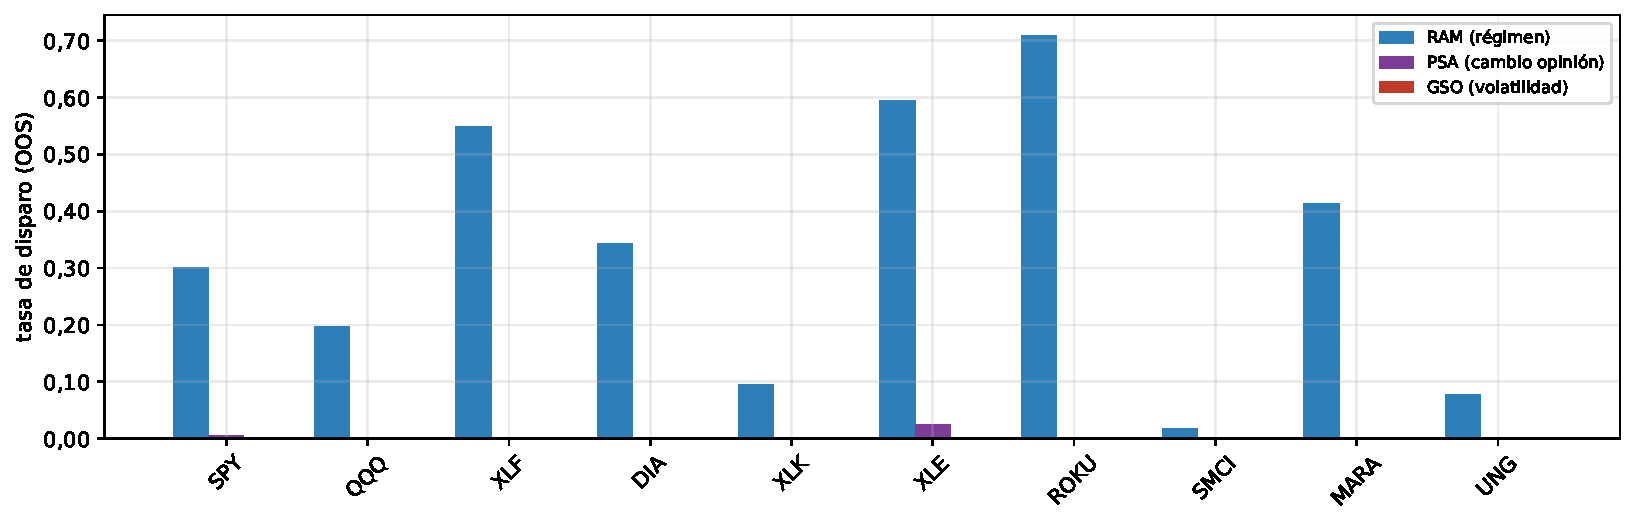
\includegraphics[width=0.82\textwidth]{figuras/cap4_activacion_panel}
\caption{Tasa de disparo de RAM, PSA y GSO y tasa de intervención de la regla, activo a activo. RAM domina en todo el panel y los otros dos apenas se encienden: la supervisión recae, como en SPY, sobre el canal del régimen.}
\label{fig:mp-activacion-panel}
\end{figure}

\begin{figure}[htbp]
\centering
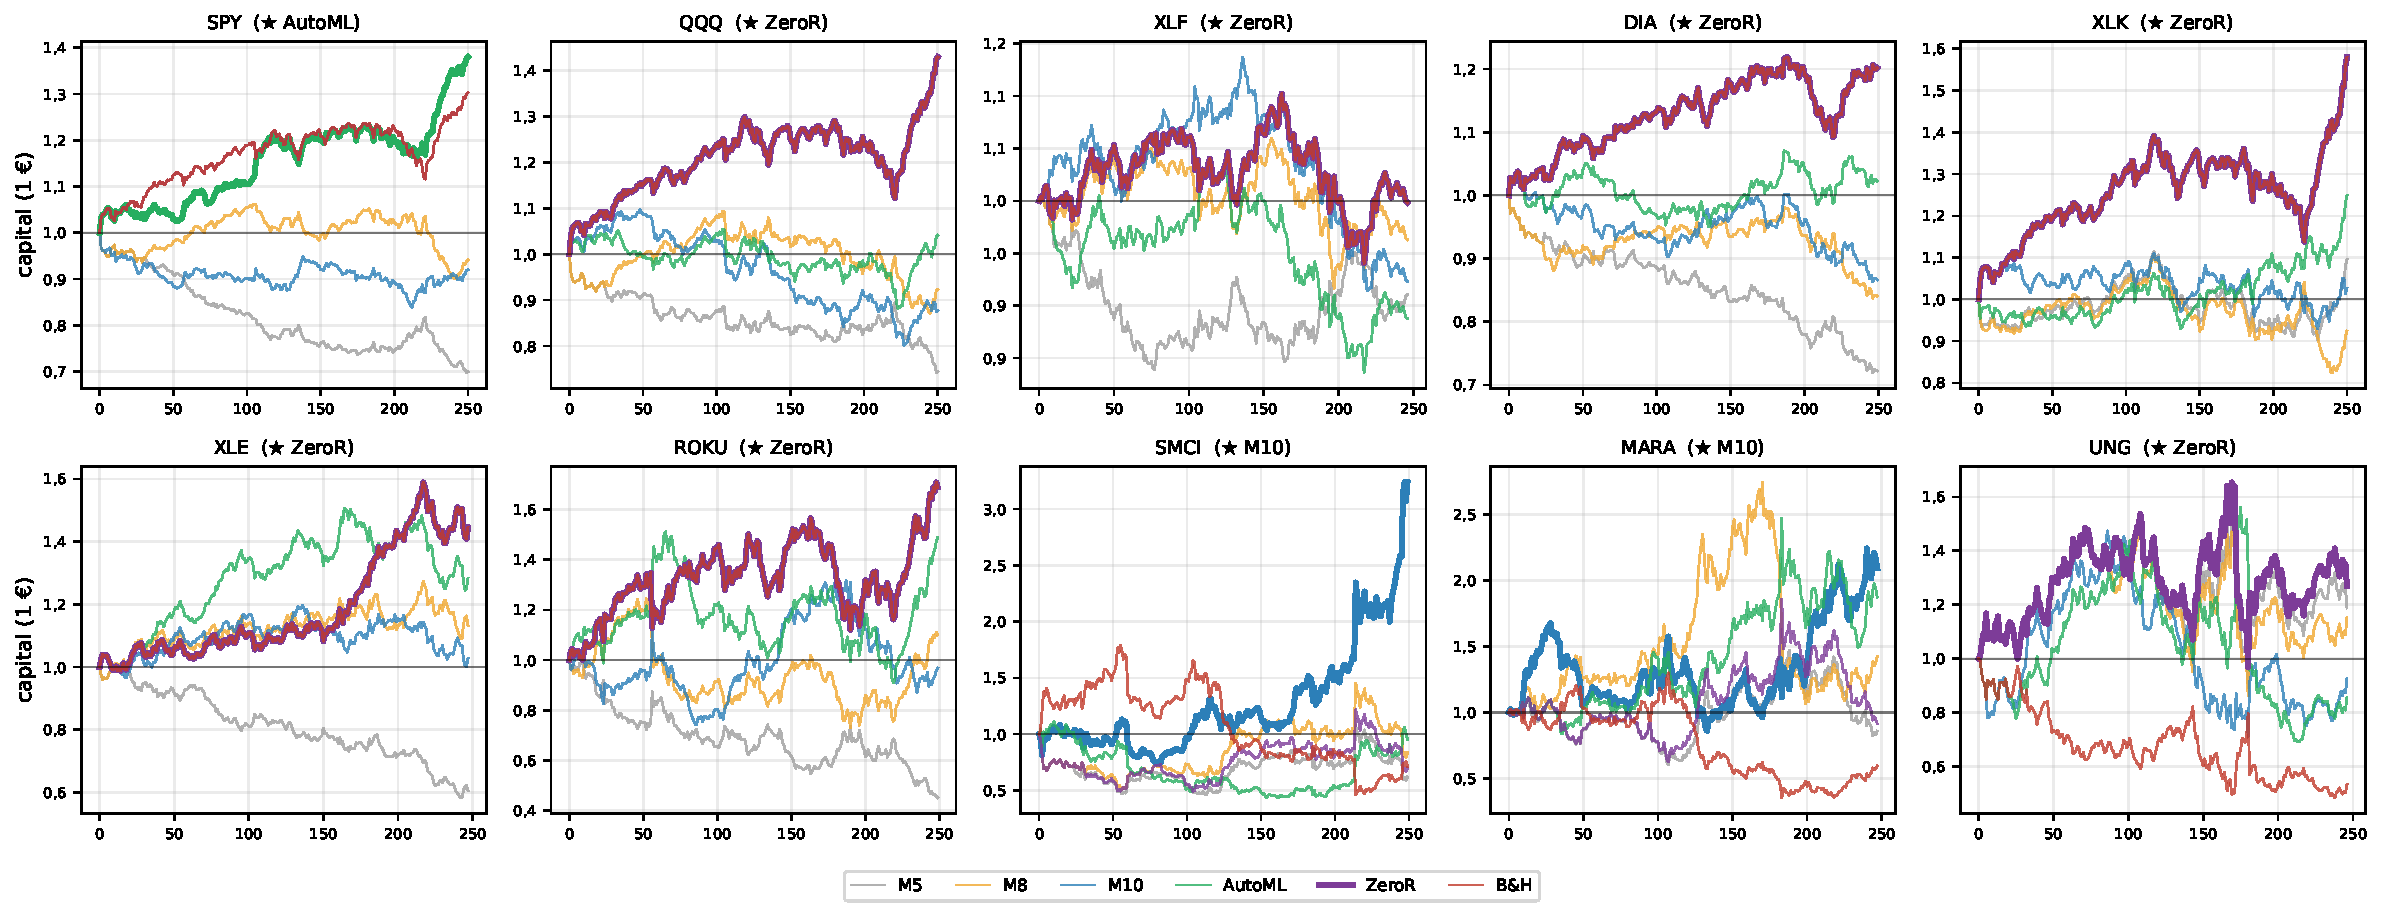
\includegraphics[width=0.78\textwidth]{figuras/cap4_equity_panel}
\caption{Curvas de capital por activo (un euro inicial), con la mejor derivada de STRATA destacada frente a las referencias. En cuatro activos una derivada bate al pasivo en Sharpe: SPY, SMCI, MARA y UNG. En SMCI/MARA/UNG el pasivo pierde o ronda el cero y la derivada saca Sharpe positivo yendo defensiva (lectura de valor direccional); en SPY la ventaja es sobre todo beta de mercado en un periodo alcista. }
\label{fig:mp-equity-panel}
\end{figure}

\begin{figure}[htbp]
\centering
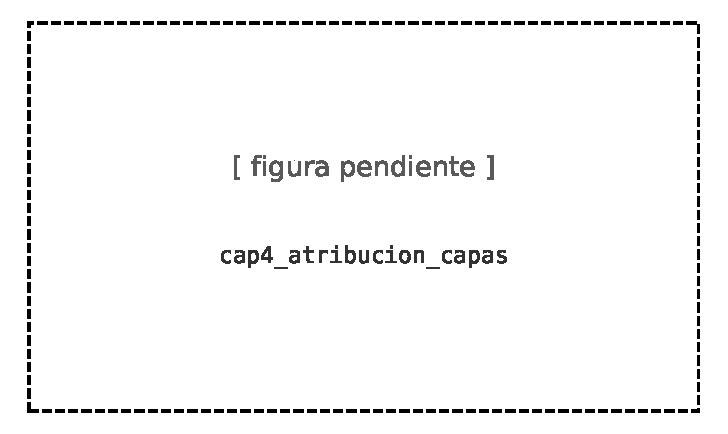
\includegraphics[width=0.74\textwidth]{figuras/cap4_atribucion_capas}
\caption{Reparto de funciones entre las dos capas. A la izquierda, atribución del P\&L de rescate por detector sobre SPY: el canal de régimen (RAM) concentra el $100\%$, PSA y GSO aportan cero. A la derecha, evolución diaria del rescate de la regla (riesgo, $\Delta$Sharpe acumulado) frente al del aprendiz (accuracy, aciertos acumulados sobre el agente): cada serie sube por un eje distinto.}
\label{fig:mp-capas}
\end{figure}

\begin{figure}[htbp]
\centering
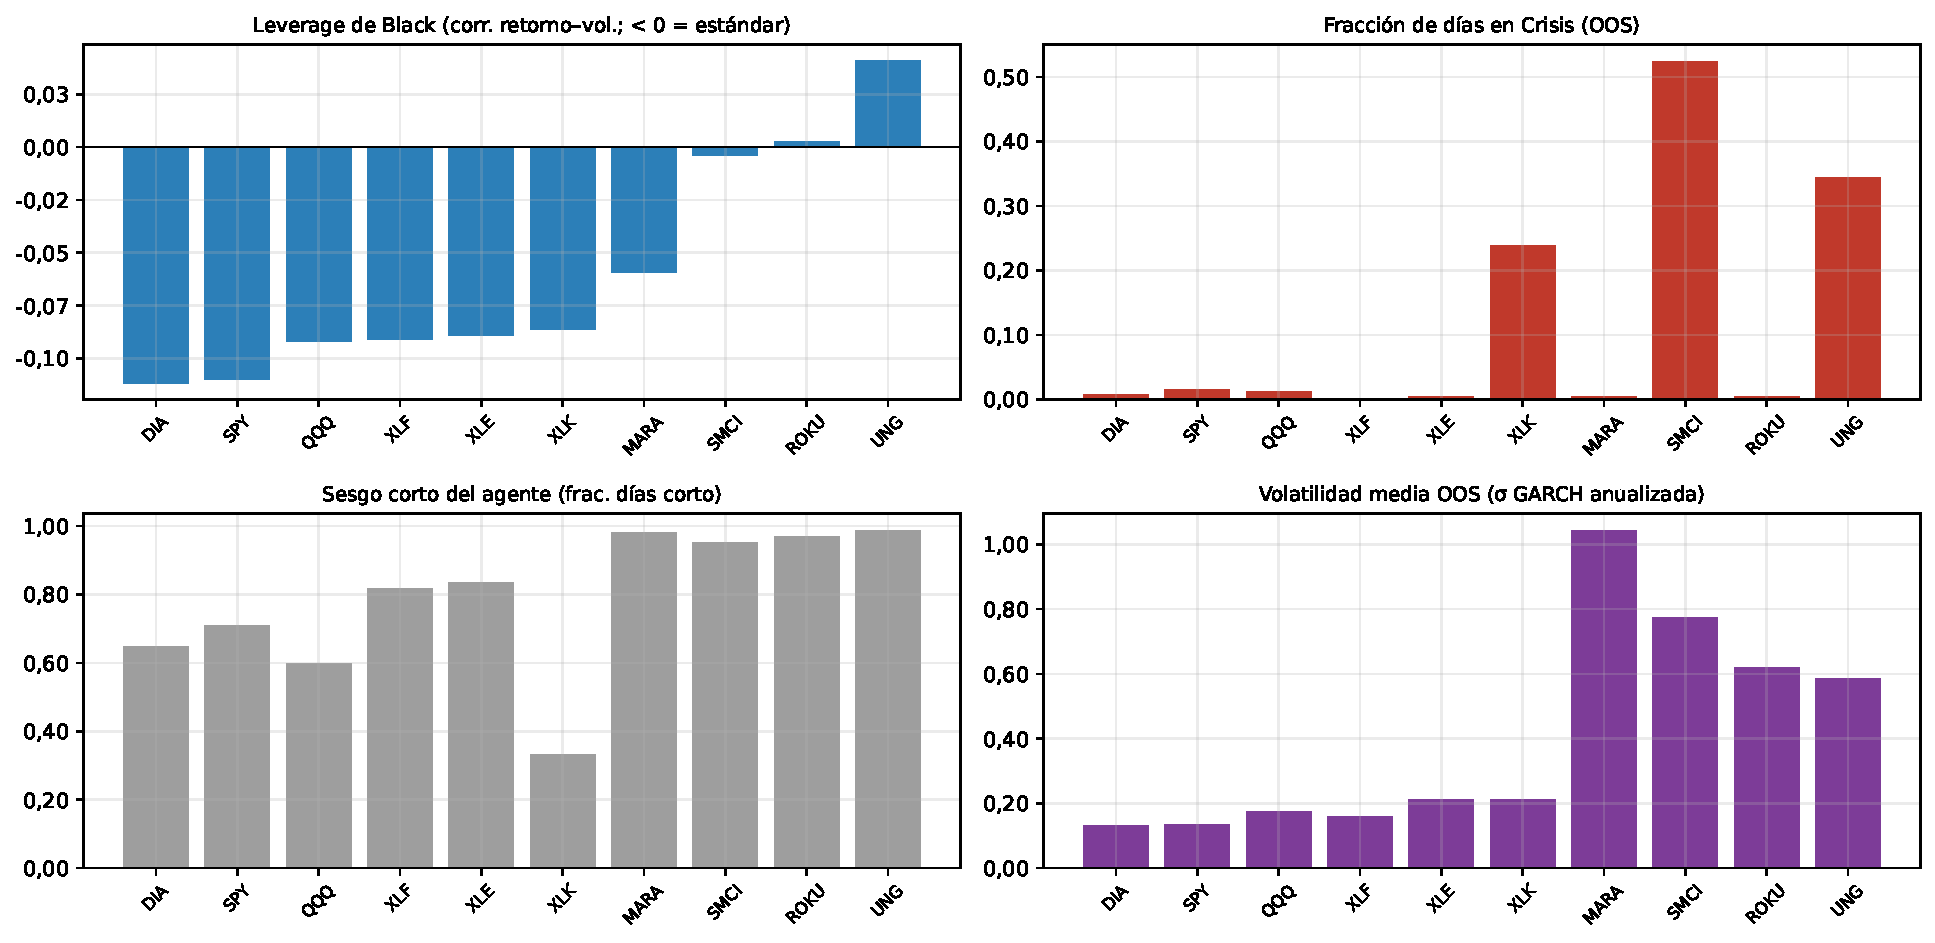
\includegraphics[width=0.82\textwidth]{figuras/cap4_naturaleza_panel}
\caption{Naturaleza de los diez activos en cuatro rasgos: \emph{leverage} de Black, fracción de días en Crisis, sesgo direccional del agente y volatilidad. Es la materia prima de la ley del \emph{leverage} y del agrupamiento: esa heterogeneidad es la que ordena el rescate.}
\label{fig:mp-naturaleza}
\end{figure}

\begin{figure}[htbp]
\centering
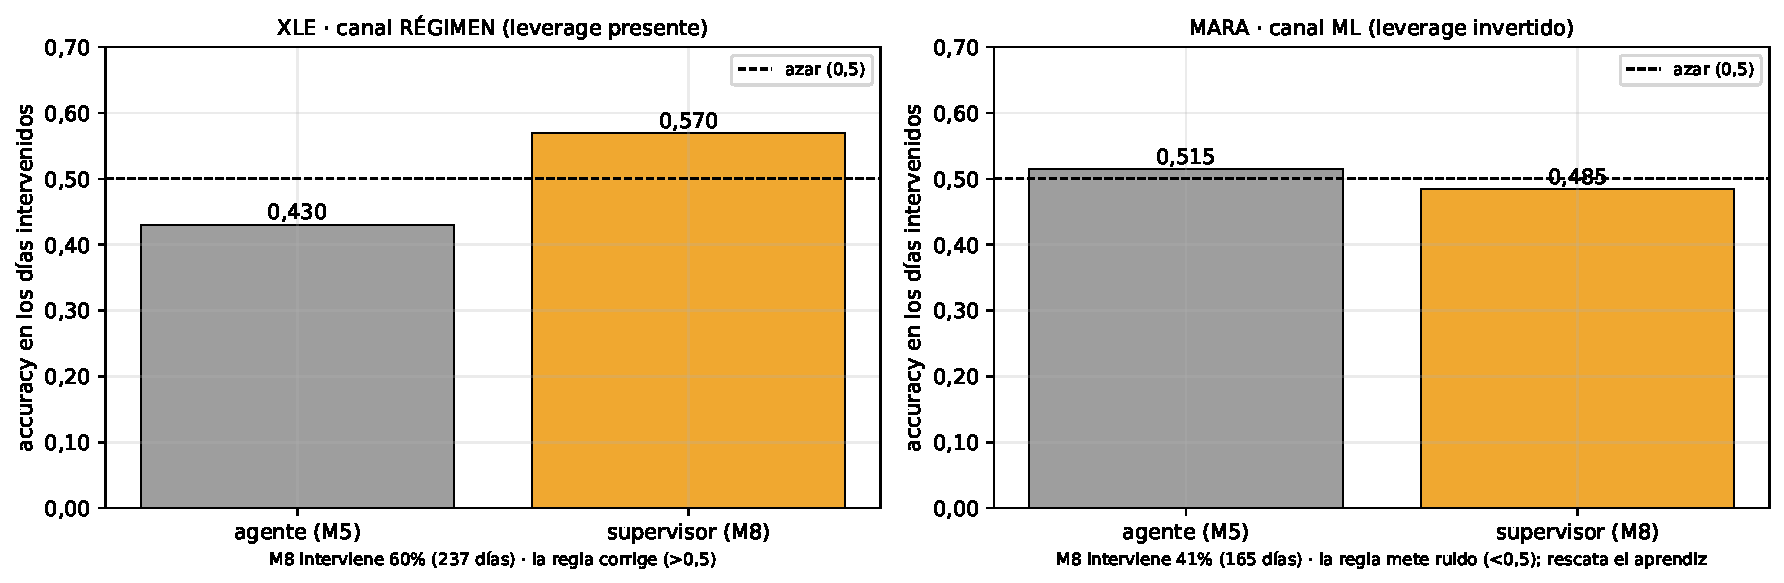
\includegraphics[width=0.74\textwidth]{figuras/cap4_casos}
\caption{Dos casos trabajados, uno por canal. A la izquierda, XLE (\emph{leverage} fuerte): el régimen es direccional y la regla rescata el riesgo del agente. A la derecha, MARA (\emph{leverage} invertido): el régimen no informa el signo y el aprendiz rescata por la vía del sesgo del agente cruzado con el régimen. Cada panel muestra la dirección del agente, la del supervisor que rescata y el régimen vigente.}
\label{fig:mp-casos}
\end{figure}

\begin{figure}[htbp]
\centering
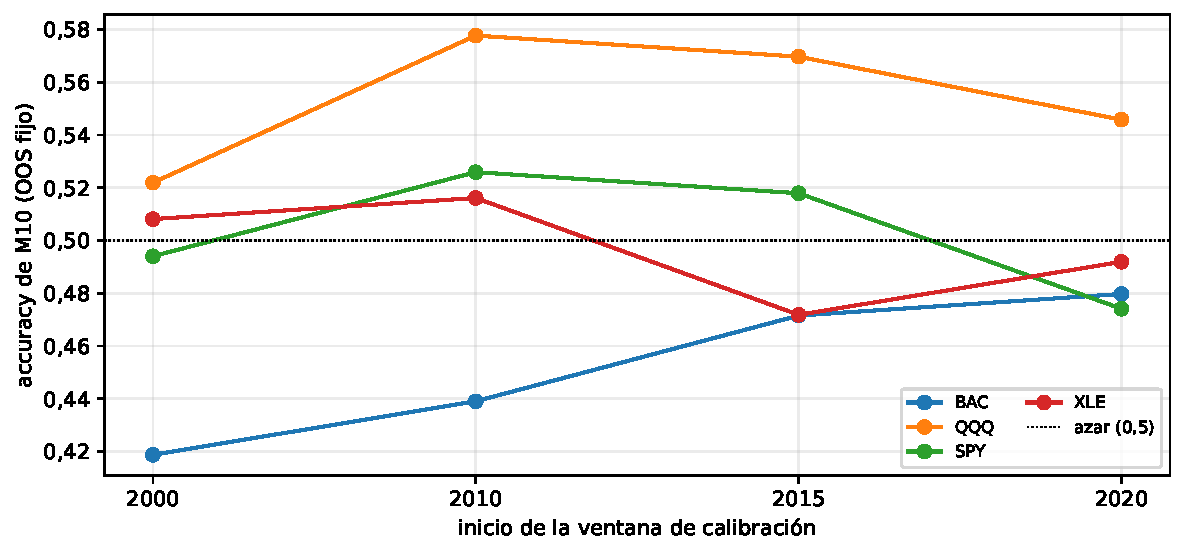
\includegraphics[width=0.74\textwidth]{figuras/cap4_robustez_calib}
\caption{Robustez a la ventana de calibración: el rescate se mantiene al desplazar el periodo con el que se cierran los umbrales de los detectores. El resultado no cuelga de una calibración concreta.}
\label{fig:mp-robustez-calib}
\end{figure}

\begin{figure}[htbp]
\centering
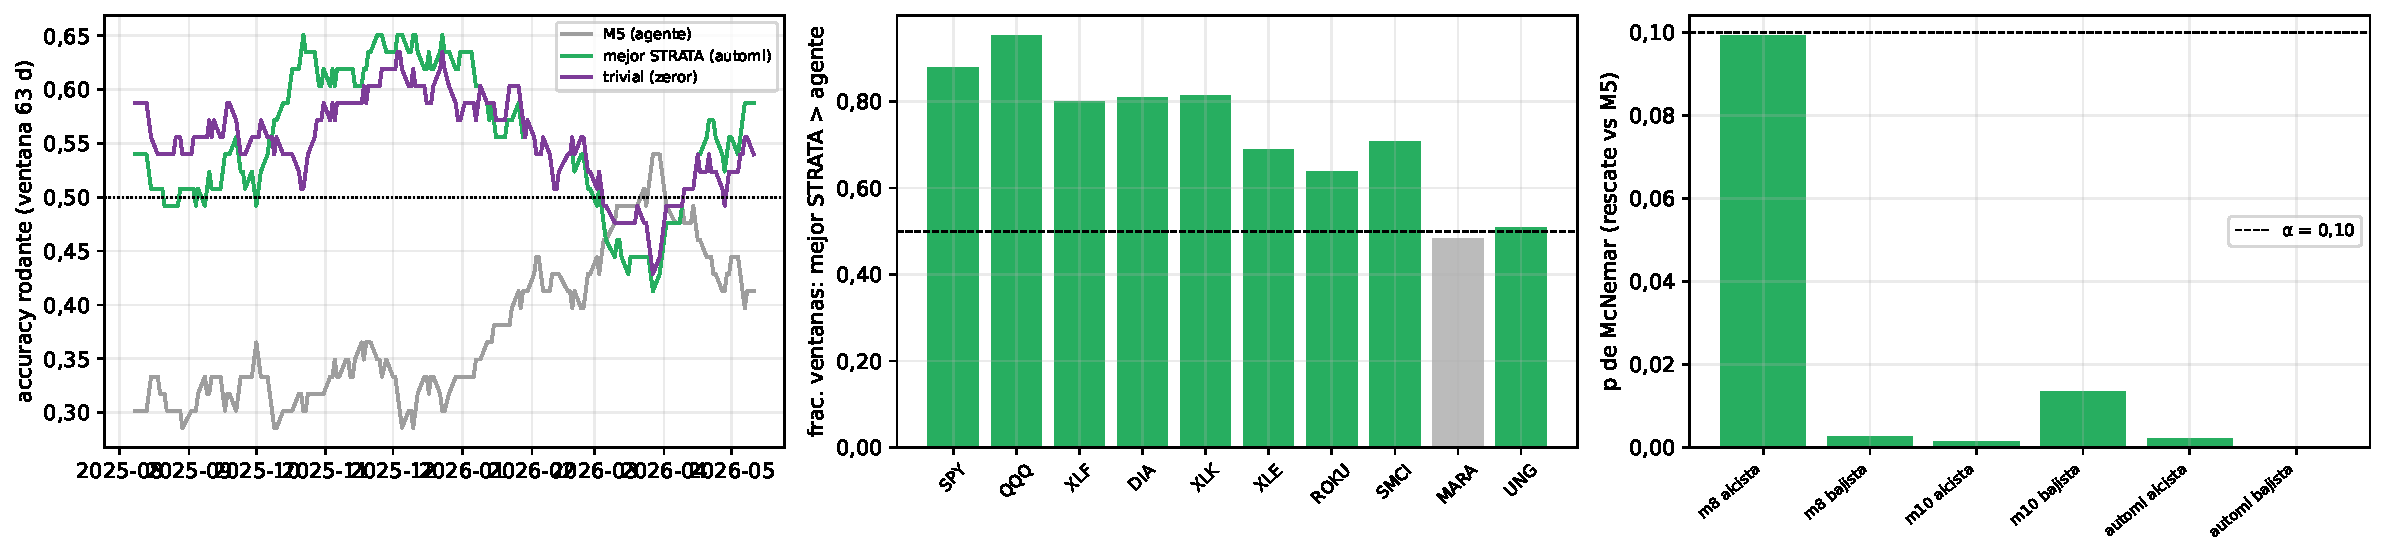
\includegraphics[width=0.85\textwidth]{figuras/cap4_robustez_panel}
\caption{Robustez del rescate en el panel por tres vías: cuota de importancia rodante en el tiempo, fracción de ventanas con rescate por activo y McNemar partido por régimen. El rescate aguanta en las tres, no es un artefacto de una ventana ni de un régimen.}
\label{fig:mp-robustez-panel}
\end{figure}

\begin{figure}[htbp]
\centering
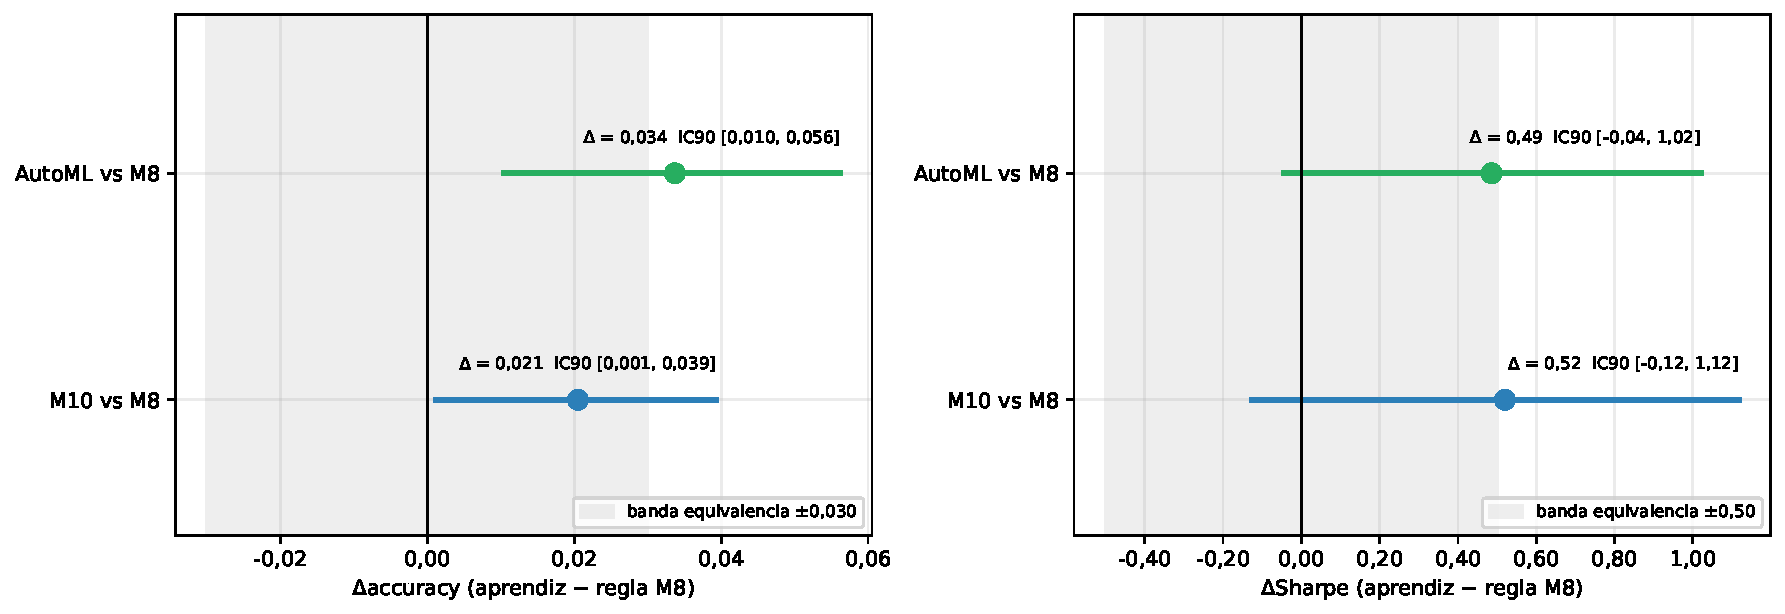
\includegraphics[width=0.58\textwidth]{figuras/cap4_tost_2x2}
\caption{Diagrama $2\times 2$ del TOST del aprendiz frente a la regla M8, ejes accuracy (horizontal) y Sharpe (vertical). Las regiones marcan superioridad, equivalencia y no concluyencia. M10 y AutoML caen en superioridad en accuracy y en no concluyencia en Sharpe: el aprendiz afina la dirección sobre la regla y empata en riesgo.}
\label{fig:mp-tost}
\end{figure}

\begin{figure}[htbp]
\centering
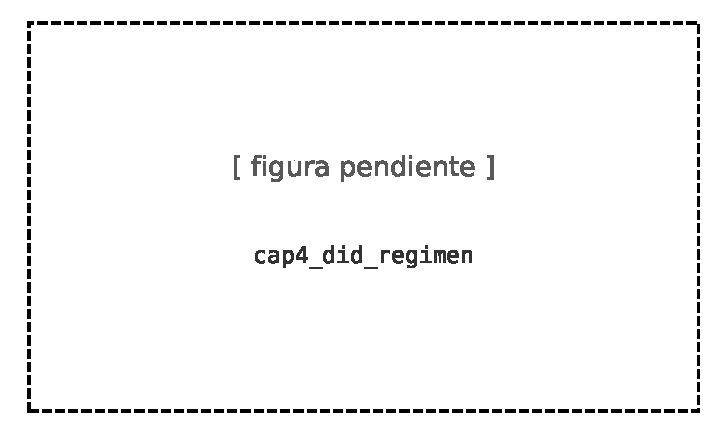
\includegraphics[width=0.58\textwidth]{figuras/cap4_did_regimen}
\caption{Complementariedad de los supervisores por régimen: $\Delta$Sharpe de M8, M10 y AutoML frente al agente, en mercado alcista y bajista. M10 rescata más en alcista, AutoML más en bajista. El contraste formal de ese reparto (diferencia en diferencias, $\Delta\Delta$Sharpe $= +1{,}37$, $p = 0{,}008$) está en la Figura~\ref{fig:anx-did}.}
\label{fig:mp-did}
\end{figure}
